\documentclass[10pt,twocolumn]{article}
\usepackage[utf8]{inputenc}
\usepackage[T1]{fontenc}
\usepackage{lmodern}
\usepackage[margin=2cm]{geometry}
\usepackage{amsmath,amssymb}
\usepackage{graphicx}
\usepackage{booktabs}
\usepackage{array}
\usepackage{xcolor}
\usepackage{caption}
\usepackage[hidelinks]{hyperref}

% Terminos en espanol sin depender de babel-spanish
\renewcommand{\abstractname}{Resumen}
\renewcommand{\figurename}{Figura}
\renewcommand{\tablename}{Tabla}
\renewcommand{\refname}{Referencias}
\renewcommand{\contentsname}{Indice}

\captionsetup{font=small,labelfont=bf}
\setlength{\parskip}{2pt}

\title{\vspace{-1.2em}\textbf{Defensa Adaptativa para APIs en el Borde mediante\\
Teor\'ia de Juegos Estoc\'asticos: equilibrando Seguridad y Sostenibilidad Energ\'etica}}
\author{Equipo \emph{Stochastic Green Edge} (SGE)\\
\small Prototipo de investigaci\'on en Ciberseguridad Cloud y Green Computing}
\date{\today}

\begin{document}
\maketitle

\begin{abstract}
\noindent La inspecci\'on profunda y sistem\'atica de todo el tr\'afico entrante hacia
una API p\'ublica ofrece m\'axima seguridad pero incurre en un costo energ\'etico
elevado y constante, en tensi\'on con los objetivos de la \emph{computaci\'on
sostenible} (Green Computing). Este trabajo propone \textbf{Stochastic Green Edge}
(SGE), un mecanismo de defensa perimetral de dos capas (\emph{Edge} ligero y
\emph{Serverless} de inspecci\'on profunda) que decide, en tiempo real y por cada
petici\'on sospechosa, si escalar a la inspecci\'on costosa. La decisi\'on se
formula como un \emph{juego estoc\'astico no cooperativo con informaci\'on
imperfecta} entre un Defensor y un Atacante, y se resuelve calculando el
\emph{Equilibrio de Nash en estrategias mixtas}. Sobre una simulaci\'on de
$3000$ peticiones con una mezcla realista ($80\%$ leg\'itimo, $15\%$ bots ruidosos,
$5\%$ ataques dirigidos) y promediando $20$ semillas, SGE alcanza una mitigaci\'on
global del $95.5\%$ y del $81.8\%$ para ataques avanzados, consumiendo un
$86.8\%$ menos de energ\'ia que el enfoque tradicional de inspecci\'on del $100\%$.
Mostramos adem\'as la frontera de compromiso seguridad--energ\'ia y c\'omo el
equilibrio de Nash concentra adaptativamente la energ\'ia costosa en el tr\'afico
de mayor riesgo.

\vspace{4pt}
\noindent\textbf{Palabras clave:} Teor\'ia de Juegos, Equilibrio de Nash,
Seguridad de APIs, Edge Computing, Serverless, Green Computing, Juegos Estoc\'asticos.
\end{abstract}

\section{Introducci\'on}
Las APIs p\'ublicas son un vector de ataque cr\'itico: reciben tr\'afico
heterog\'eneo que combina usuarios leg\'itimos, bots automatizados ruidosos y
adversarios dirigidos y sigilosos. La pr\'actica habitual de someter cada
petici\'on a una inspecci\'on profunda (sanitizaci\'on exhaustiva, validaci\'on
criptogr\'afica, an\'alisis de payload) maximiza la detecci\'on pero impone un
consumo de CPU y energ\'ia elevado y \emph{constante}, independientemente del
riesgo real de cada petici\'on. Este patr\'on entra en conflicto directo con la
computaci\'on sostenible, que busca minimizar los ciclos de c\'omputo y la huella
energ\'etica~\cite{green}.

La observaci\'on central de este trabajo es que la mayor\'ia del tr\'afico no
justifica el costo de la inspecci\'on profunda: el tr\'afico leg\'itimo debe
servirse con energ\'ia m\'inima y los bots ruidosos pueden frenarse de forma barata
en el borde mediante \emph{rate-limiting}. \'Unicamente una fracci\'on peque\~na y
sigilosa (ataques dirigidos que imitan tr\'afico leg\'itimo) requiere realmente la
capa costosa. El problema es que esa fracci\'on \textbf{no es observable} de forma
directa: el defensor opera bajo \emph{informaci\'on imperfecta}.

Proponemos modelar la decisi\'on de escalado como un juego no cooperativo entre el
Defensor y el Atacante y resolver el \emph{Equilibrio de Nash en estrategias
mixtas}, obteniendo una pol\'itica de escalado \emph{aleatorizada} que es \'optima
en el sentido de la teor\'ia de juegos: ninguna de las partes puede mejorar su
utilidad esperada desviándose unilateralmente. Nuestras contribuciones son:
\begin{itemize}\itemsep2pt
  \item Una arquitectura perimetral de dos capas (Edge + Serverless) con un modelo
        de costo energ\'etico expl\'icito, incluida la penalizaci\'on por
        \emph{Cold Start}.
  \item La formulaci\'on del escalado como un juego bimatriz $2\times 2$ y un motor
        que calcula su Equilibrio de Nash en estrategias mixtas por enumeraci\'on
        de soportes.
  \item Una evaluaci\'on emp\'irica reproducible que cuantifica el compromiso
        seguridad--energ\'ia frente a l\'ineas base y traza su frontera de Pareto.
\end{itemize}

\section{Trabajo relacionado}
La teor\'ia de juegos se ha aplicado extensamente a la seguridad
(\emph{security games}), modelando la asignaci\'on de recursos de defensa frente a
un adversario racional~\cite{tambe,alpcan}. Los \emph{juegos estoc\'asticos} de
Shapley~\cite{shapley} y su extensi\'on a informaci\'on imperfecta capturan
entornos donde el estado evoluciona y los jugadores no observan por completo las
acciones del rival. El concepto de \emph{Equilibrio de Nash}~\cite{nash} en
estrategias mixtas es la soluci\'on est\'andar cuando no existe un equilibrio en
estrategias puras, como ocurre en interacciones de tipo \emph{matching pennies}.
Paralelamente, la computaci\'on sostenible y el \emph{cómputo consciente de la
energ\'ia}~\cite{green} promueven arquitecturas que ajustan din\'amicamente el
gasto de recursos. Nuestro trabajo sit\'ua la decisi\'on de inspecci\'on profunda
en la intersecci\'on de ambos campos: usa el equilibrio de Nash como criterio para
gastar energ\'ia \emph{solo cuando el riesgo esperado lo justifica}.

\section{Modelo del sistema}
\label{sec:model}
SGE simula dos capas de infraestructura cloud (Figura~\ref{fig:energy} ilustra su
costo relativo):

\paragraph{Capa Edge (filtro ligero).} Funci\'on de paso r\'apido con costo
energ\'etico m\'inimo ($C_{\text{edge}}=1$ unidad). Extrae m\'etricas baratas de la
petici\'on HTTP ---frecuencia de la IP de origen, tama\~no del payload, anomal\'ia
del \emph{User-Agent} y anomal\'ia estructural del payload--- y ejecuta el
\emph{cerebro matem\'atico} (el motor de Nash). Aplica adem\'as \emph{rate-limiting}
que frena los bots ruidosos (alta frecuencia de IP y firma de agente an\'omala) sin
invocar la capa costosa. Los ataques avanzados imitan tr\'afico leg\'itimo y
\emph{no} son detenidos aqu\'i.

\paragraph{Capa Serverless (inspecci\'on profunda).} Funci\'on robusta que realiza
sanitizaci\'on exhaustiva y validaci\'on criptogr\'afica del payload. Permanece
inactiva salvo que el modelo decida activarla. Su costo de ejecuci\'on es
$C_{\text{exec}}=15$ unidades y, tras un periodo de inactividad, incurre en
\emph{Cold Start} con costo $C_{\text{cold}}=25$ unidades. Cuando se invoca,
detecta de forma fiable cualquier clase de ataque.

Los valores de energ\'ia (Joules/ciclos relativos) siguen la relaci\'on
$C_{\text{edge}}:C_{\text{exec}}:C_{\text{cold}} = 1:15:25$, reflejando el elevado
sobrecoste de la inspecci\'on profunda y el arranque en fr\'io t\'ipico del c\'omputo
sin servidor.

\section{Formulaci\'on como juego}
\label{sec:game}
Modelamos cada petici\'on \emph{sospechosa} como una interacci\'on de un solo tiro
(una etapa del juego estoc\'astico) entre dos jugadores.

\paragraph{Jugadores y acciones.}
El \textbf{Defensor} elige entre dos estrategias puras:
\begin{itemize}\itemsep1pt
  \item $D_V$ (\emph{Verde}): permanecer en la capa Edge (energ\'ia m\'inima).
  \item $D_A$ (\emph{Activa}): escalar a la inspecci\'on Serverless.
\end{itemize}
El \textbf{Atacante} elige entre:
\begin{itemize}\itemsep1pt
  \item $A_L$ (\emph{Ligero}): ataque ruidoso/automatizado.
  \item $A_M$ (\emph{Avanzado}): ataque dirigido y sigiloso.
\end{itemize}
El Defensor juega $D_V$ con probabilidad $p$ y $D_A$ con probabilidad $1-p$; el
Atacante juega $A_L$ con probabilidad $q$ y $A_M$ con $1-q$.

\paragraph{Funci\'on de utilidad del Defensor.}
La utilidad del Defensor ante el par de acciones $(a,d)$ es
\begin{equation}
\label{eq:util}
U_D(a,d) = \alpha\, R(a,d) \;-\; \beta\, C_{\text{energy}}(d) \;-\; \gamma\, C_{\text{damage}}(a,d),
\end{equation}
donde $R$ es la recompensa por detecci\'on o por procesar tr\'afico leg\'itimo con
energ\'ia m\'inima, $C_{\text{energy}}$ es el costo energ\'etico de la acci\'on
defensiva, $C_{\text{damage}}$ penaliza severamente que un ataque avanzado evada la
seguridad por quedarse en el borde, y $\alpha,\beta,\gamma \ge 0$ son pesos de
ponderaci\'on configurables.

\paragraph{Modulaci\'on por sospecha (informaci\'on imperfecta).}
El Defensor no observa la clase real de la petici\'on; solo infiere una
\emph{puntuaci\'on de sospecha} $s\in[0,1]$ a partir de las m\'etricas del Edge, con
la anomal\'ia de payload como se\~nal dominante (es lo que solo la inspecci\'on
profunda puede detectar):
\begin{equation}
s = 0.15\,\phi_{\text{ip}} + 0.15\,\phi_{\text{ua}} + 0.70\,\phi_{\text{payload}},
\end{equation}
siendo $\phi_{\text{ip}}=1-e^{-\text{freq}/6}$ la saturaci\'on de la frecuencia de
IP. La sospecha escala el riesgo, $\rho = s_0 + (1-s_0)\,s$ con piso $s_0=0.15$, y
con \'el la severidad del da\~no $C_{\text{damage}}=D_0\,\rho$ y la ganancia de
brecha del atacante. As\'i, el equilibrio resultante es \emph{espec\'ifico de cada
petici\'on}.

\paragraph{Matrices de pago.}
Con los par\'ametros del prototipo ($\alpha=\beta=\gamma=1$, $R_{\text{edge}}=10$,
$R_{\text{deep}}=12$, $D_0=140$, ganancia de brecha $G_0=200$, costo de ataque
avanzado $K=20$, penalizaciones de detecci\'on $5$ y $15$) se construyen las
matrices del Defensor $\mathbf{A}$ y del Atacante $\mathbf{B}$ (filas $D_V,D_A$;
columnas $A_L,A_M$):
\begin{align}
A_{D_V,A_L} &= \alpha R_{\text{edge}} - \beta C_{\text{edge}} \\
A_{D_V,A_M} &= -\beta C_{\text{edge}} - \gamma C_{\text{damage}} \\
A_{D_A,\cdot} &= \alpha R_{\text{deep}} - \beta C_{\text{serverless}}
\end{align}
El pago $(D_V,A_M)$ es fuertemente negativo (brecha), mientras que $D_A$ neutraliza
el ataque a costa de energ\'ia. Esta estructura es de tipo \emph{matching pennies}:
el Defensor prefiere $D_V$ frente a $A_L$ pero $D_A$ frente a $A_M$, y el Atacante
prefiere $A_M$ frente a $D_V$ pero $A_L$ frente a $D_A$. En consecuencia \emph{no
existe equilibrio en estrategias puras} y la soluci\'on es un equilibrio
completamente mixto.

\section{Equilibrio de Nash en estrategias mixtas}
\label{sec:nash}
En un juego bimatriz $2\times2$ sin equilibrio puro, el equilibrio mixto se obtiene
por el \emph{principio de indiferencia}: cada jugador aleatoriza de modo que su
rival sea indiferente entre sus dos acciones.

La probabilidad $p$ (jugar $D_V$) hace al Atacante indiferente entre $A_L$ y $A_M$:
\begin{equation}
p\,B_{D_V,A_L} + (1-p)B_{D_A,A_L} = p\,B_{D_V,A_M} + (1-p)B_{D_A,A_M},
\end{equation}
\begin{equation}
\label{eq:p}
p = \frac{B_{D_A,A_M}-B_{D_A,A_L}}{(B_{D_V,A_L}-B_{D_A,A_L})-(B_{D_V,A_M}-B_{D_A,A_M})}.
\end{equation}
An\'alogamente, $q$ (jugar $A_L$) hace al Defensor indiferente entre $D_V$ y $D_A$:
\begin{equation}
\label{eq:q}
q = \frac{A_{D_A,A_M}-A_{D_V,A_M}}{(A_{D_V,A_L}-A_{D_V,A_M})-(A_{D_A,A_L}-A_{D_A,A_M})}.
\end{equation}
El motor (\texttt{sge/game\_theory.py}) implementa la enumeraci\'on de soportes:
primero busca el equilibrio interior mixto por
\eqref{eq:p}--\eqref{eq:q} y, si no es v\'alido ($p,q\notin[0,1]$), recurre a un
equilibrio en estrategias puras por mejor respuesta mutua. Como validaci\'on, para
el juego de \emph{matching pennies} el motor devuelve $p=q=0.5$.

\paragraph{Ejemplo resuelto.}
Para una petici\'on con alta anomal\'ia de payload ($s=0.712$), las matrices son
\[
\mathbf{A}=\begin{pmatrix} 9.00 & -106.73\\ -3.00 & -3.00 \end{pmatrix},\quad
\mathbf{B}=\begin{pmatrix} -5.00 & 131.04\\ -5.00 & -35.00 \end{pmatrix}.
\]
Aplicando \eqref{eq:p}--\eqref{eq:q} se obtiene el equilibrio mixto
$p=0.181$ (jugar Verde) y $q=0.896$: el Defensor \textbf{escala a Serverless con
probabilidad $1-p=0.819$}, concentrando la energ\'ia en el tr\'afico de alto riesgo.
La Figura~\ref{fig:response} muestra c\'omo la probabilidad de escalado crece
mon\'otonamente con la sospecha.

\begin{figure}[t]
\centering
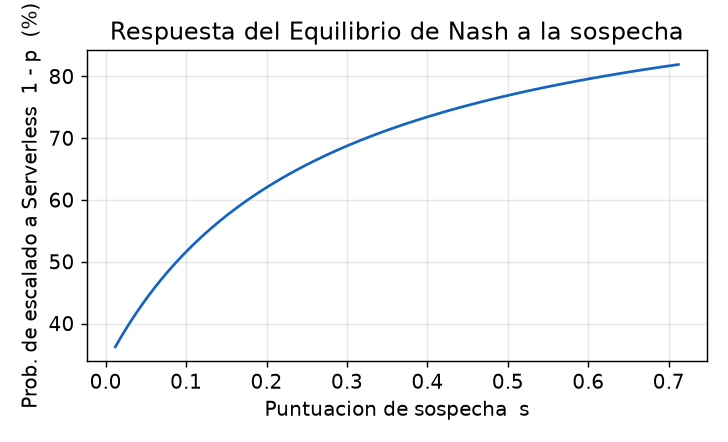
\includegraphics[width=\linewidth]{figures/fig3_response.png}
\caption{Respuesta del Equilibrio de Nash: probabilidad de escalar a la capa
Serverless ($1-p$) en funci\'on de la puntuaci\'on de sospecha $s$. El escalado es
despreciable para tr\'afico benigno y crece con la anomal\'ia del payload.}
\label{fig:response}
\end{figure}

\section{Metodolog\'ia experimental}
\label{sec:method}
\paragraph{Generaci\'on de tr\'afico.} Simulamos un flujo constante con la mezcla
$80\%$ usuarios leg\'itimos, $15\%$ bots ruidosos ($A_L$) y $5\%$ hackers dirigidos
($A_M$). Los leg\'itimos usan IP diversa, agente de navegador y payload peque\~no y
limpio; los bots concentran pocas IPs (alta frecuencia) con agentes an\'omalos
(\texttt{curl}, \texttt{sqlmap}); los avanzados usan agente cuasi-normal y payload
voluminoso con \emph{tokens} de inyecci\'on.

\paragraph{L\'ineas base.}
Comparamos SGE (Adaptativo) contra: (i) \textbf{Tradicional}, que inspecciona el
$100\%$ del tr\'afico en Serverless (m\'axima seguridad, energ\'ia
$C_{\text{cold}} + (n-1)C_{\text{exec}}$); y (ii) \textbf{Edge-only}, que nunca
escala (energ\'ia m\'inima $n\,C_{\text{edge}}$ pero $0\%$ de mitigaci\'on de
ataques avanzados).

\paragraph{M\'etricas.} Tasa de mitigaci\'on global y de ataques avanzados, energ\'ia
total consumida (Joules simulados) y energ\'ia ahorrada frente al enfoque
tradicional. Reportamos media y desviaci\'on est\'andar sobre $20$ semillas con
$n=3000$ peticiones. Todos los experimentos son reproducibles mediante
\texttt{python3 paper/run\_experiments.py}.

\section{Resultados}
\label{sec:results}
La Tabla~\ref{tab:main} resume la comparaci\'on principal. SGE mitiga el
$95.5\%$ del total de ataques y el $81.8\%$ de los ataques avanzados, mientras
reduce el consumo energ\'etico en un $\mathbf{86.8\%}$ respecto al enfoque
tradicional (de $45{,}010$ a $\sim\!5{,}922$ Joules). El enfoque Edge-only, aunque
minimiza la energ\'ia, deja pasar la totalidad de los ataques avanzados
($0\%$ de mitigaci\'on), lo que confirma que la capa profunda es imprescindible
para la fracci\'on sigilosa.

\begin{table}[t]
\centering
\small
\caption{Comparaci\'on de enfoques (media $\pm$ desv.\ est.\ sobre $20$ semillas,
$n=3000$). Energ\'ia en Joules simulados.}
\label{tab:main}
\begin{tabular}{lccc}
\toprule
\textbf{Enfoque} & \textbf{Mit.\ global} & \textbf{Mit.\ avanz.} & \textbf{Energ\'ia} \\
\midrule
Tradicional (100\%) & $100\%$ & $100\%$ & $45{,}010$ \\
\textbf{Adaptativo (Nash)} & $\mathbf{95.5}\%$ & $\mathbf{81.8}\%$ & $\mathbf{5{,}922}$ \\
Edge-only (0\%) & $74.0\%$ & $0\%$ & $3{,}000$ \\
\bottomrule
\end{tabular}
\end{table}

\begin{figure}[t]
\centering
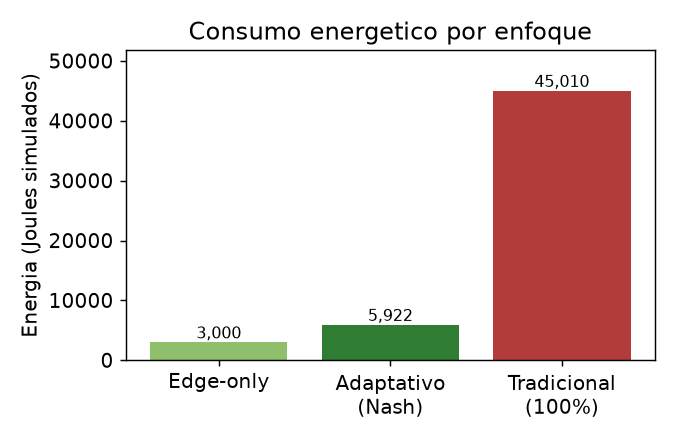
\includegraphics[width=\linewidth]{figures/fig1_energy.png}
\caption{Consumo energ\'etico por enfoque. El Adaptativo se sit\'ua cerca del piso
del Edge-only, muy por debajo del Tradicional.}
\label{fig:energy}
\end{figure}

\paragraph{Frontera de compromiso.}
La Figura~\ref{fig:pareto} traza la frontera seguridad--energ\'ia al variar el
incentivo de brecha asumido para el adversario ($G_0$, que representa el valor de la
API). A mayor incentivo, el equilibrio de Nash prescribe m\'as escalado y por tanto
mayor mitigaci\'on de ataques avanzados a costa de m\'as energ\'ia, aproxim\'andose
asint\'oticamente al punto Tradicional. Es notable que incluso en su extremo m\'as
seguro ($\sim\!93\%$ de mitigaci\'on avanzada) el Adaptativo consume del orden de
$6{,}300$ Joules, un orden de magnitud menos que los $45{,}010$ del Tradicional.

\begin{figure}[t]
\centering
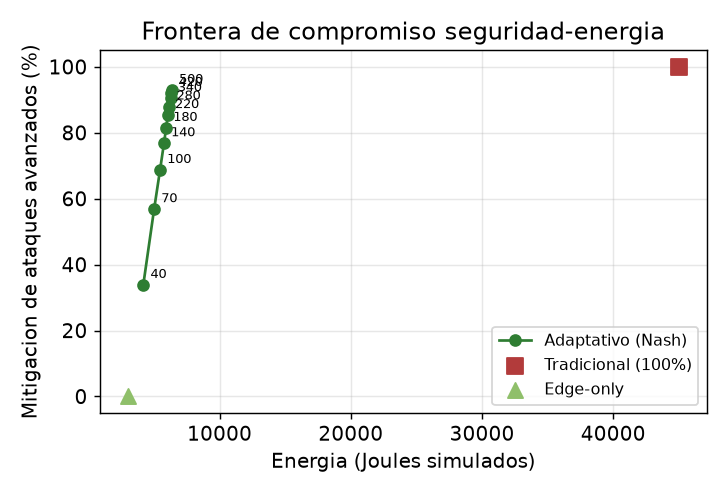
\includegraphics[width=\linewidth]{figures/fig2_pareto.png}
\caption{Frontera de Pareto seguridad--energ\'ia del enfoque Adaptativo al variar el
incentivo de brecha $G_0$ (etiquetas junto a cada punto), con los puntos de
referencia Tradicional y Edge-only.}
\label{fig:pareto}
\end{figure}

\section{Discusi\'on}
\label{sec:discussion}
Los resultados evidencian que aleatorizar la decisi\'on de inspecci\'on seg\'un el
Equilibrio de Nash captura la mayor parte del valor de seguridad de la inspecci\'on
exhaustiva con una fracci\'on de su costo energ\'etico. La clave es la
\emph{especializaci\'on por capa}: el Edge neutraliza gratis a los bots ruidosos y
el juego reserva la energ\'ia de Serverless para el tr\'afico con anomal\'ia de
payload, que es donde la inspecci\'on profunda aporta valor.

Una propiedad te\'orica relevante es que, en el equilibrio mixto, la probabilidad de
escalado $p$ queda determinada por la matriz de pagos del \emph{Atacante}
(ecuaci\'on~\eqref{eq:p}): es el incentivo del adversario ---no la mera aversi\'on
al riesgo del defensor--- lo que fija el nivel \'optimo de aleatorizaci\'on. Esto es
deseable, pues vincula el gasto de recursos a la amenaza racional esperada.

\paragraph{Limitaciones.} (i) El modelo de detecci\'on de Serverless es idealizado
(detecci\'on perfecta al inspeccionar); introducir falsos negativos/positivos es
trabajo futuro. (ii) Cada petici\'on se trata como una etapa independiente; un
verdadero juego estoc\'astico multi-etapa con estado (reputaci\'on de IP,
calentamiento de Serverless) permitir\'ia pol\'iticas dependientes de la historia.
(iii) La puntuaci\'on de sospecha usa heur\'isticas ligeras; aprenderla con datos
reales mejorar\'ia la calibraci\'on. (iv) Los costos energ\'eticos son unidades
relativas simuladas, no mediciones f\'isicas.

\section{Conclusiones}
\label{sec:conclusion}
Presentamos SGE, una defensa perimetral adaptativa para APIs que formula la
decisi\'on de inspecci\'on profunda como un juego estoc\'astico no cooperativo con
informaci\'on imperfecta y la resuelve mediante el Equilibrio de Nash en estrategias
mixtas. Emp\'iricamente, SGE logra un $95.5\%$ de mitigaci\'on global y un $81.8\%$
de mitigaci\'on de ataques avanzados con un $86.8\%$ de ahorro energ\'etico frente a
la inspecci\'on total, y expone una frontera de Pareto sintonizable seg\'un el valor
de la API. El enfoque muestra que la teor\'ia de juegos es una herramienta efectiva
para alinear la seguridad con los objetivos de la computaci\'on sostenible. Como
trabajo futuro proponemos extender el modelo a un juego estoc\'astico multi-etapa
con estado y aprender tanto la funci\'on de sospecha como los par\'ametros de
utilidad a partir de trazas de tr\'afico reales.

\begin{thebibliography}{9}
\small
\bibitem{nash} J.~Nash. \emph{Non-Cooperative Games}. Annals of Mathematics, 54(2):286--295, 1951.
\bibitem{shapley} L.~S.~Shapley. \emph{Stochastic Games}. PNAS, 39(10):1095--1100, 1953.
\bibitem{tambe} M.~Tambe. \emph{Security and Game Theory: Algorithms, Deployed Systems, Lessons Learned}. Cambridge University Press, 2011.
\bibitem{alpcan} T.~Alpcan and T.~Ba\c{s}ar. \emph{Network Security: A Decision and Game-Theoretic Approach}. Cambridge University Press, 2010.
\bibitem{green} A.~Katal, S.~Dahiya, and T.~Choudhury. \emph{Energy efficiency in cloud computing data centers: a survey on software technologies}. Cluster Computing, 26:1845--1875, 2023.
\end{thebibliography}

\end{document}
